\documentclass[letterpaper,9pt,twoside,printwatermark=false]{pinp}

%% Some pieces required from the pandoc template
\providecommand{\tightlist}{%
  \setlength{\itemsep}{0pt}\setlength{\parskip}{0pt}}

% Use the lineno option to display guide line numbers if required.
% Note that the use of elements such as single-column equations
% may affect the guide line number alignment.

\usepackage[T1]{fontenc}
\usepackage[utf8]{inputenc}

% The geometry package layout settings need to be set here...
\geometry{layoutsize={0.95588\paperwidth,0.98864\paperheight},%
          layouthoffset=0.02206\paperwidth,%
		  layoutvoffset=0.00568\paperheight}

\definecolor{pinpblue}{HTML}{185FAF}  % imagecolorpicker on blue for new R logo
\definecolor{pnasbluetext}{RGB}{101,0,0} %



\title{DALITE Q7 - Two Sample Inference. Solutions.}

\author[a]{EPIB607 - Inferential Statistics}

  \affil[a]{Fall 2018, McGill University}

\setcounter{secnumdepth}{5}

% Please give the surname of the lead author for the running footer
\leadauthor{Bhatnagar and Hanley}

% Keywords are not mandatory, but authors are strongly encouraged to provide them. If provided, please include two to five keywords, separated by the pipe symbol, e.g:
 \keywords{  Two sample means |  Two sample proportions  }  

\begin{abstract}
This DALITE quiz will cover two sample inference. This builds on the one
sample inference we have seen so far.
\end{abstract}

\dates{This version was compiled on \today}
\doi{\url{https://sahirbhatnagar.com/EPIB607/}}

\pinpfootercontents{DALITE Q7 due November 7, 2018 by 5pm}

\begin{document}

% Optional adjustment to line up main text (after abstract) of first page with line numbers, when using both lineno and twocolumn options.
% You should only change this length when you've finalised the article contents.
\verticaladjustment{-2pt}

\maketitle
\thispagestyle{firststyle}
\ifthenelse{\boolean{shortarticle}}{\ifthenelse{\boolean{singlecolumn}}{\abscontentformatted}{\abscontent}}{}

% If your first paragraph (i.e. with the \dropcap) contains a list environment (quote, quotation, theorem, definition, enumerate, itemize...), the line after the list may have some extra indentation. If this is the case, add \parshape=0 to the end of the list environment.


\section{A researcher who wished to test the difference of two
(independent) y-bars with reported SEMs, SE0 and SE1 , did so by
computing which test
statistic?}\label{a-researcher-who-wished-to-test-the-difference-of-two-independent-y-bars-with-reported-sems-se0-and-se1-did-so-by-computing-which-test-statistic}

\begin{enumerate}
\def\labelenumi{\alph{enumi}.}
\tightlist
\item
  (ybar1 - ybar0) / (SE1 + SE0)
\item
  (ybar1 - ybar0) / (SE1 - SE0)
\item
  \textbf{(ybar1 - ybar0) / sqrt( (SE1)2 + (SE0)2 ) (Correct)}
\item
  (ybar1 - ybar0) / sqrt( (SE1)2 - (SE0)2 )
\end{enumerate}

\subsection{Correct rationales}\label{correct-rationales}

\subsection{Incorrect rationales}\label{incorrect-rationales}

\section{Which distribution is closer to Normal
?}\label{which-distribution-is-closer-to-normal}

\begin{enumerate}
\def\labelenumi{\alph{enumi}.}
\tightlist
\item
  Body weights of (unrelated) male air passengers
\item
  Body weights of (unrelated) female air passengers
\item
  \textbf{Sum of weights of a (random male, random female) pair
  (Correct)}
\item
  \textbf{Difference of weights of a (random male, random female) pair
  (Correct)}
\end{enumerate}

\subsection{Correct rationales}\label{correct-rationales-1}

\subsection{Incorrect rationales}\label{incorrect-rationales-1}

\section{\texorpdfstring{Refer to the Table on ``Postoperative Effect on
Plasma Ascorbic Acid for 105 Cases; Readings on the Same Individuals''.
You would get contradictory answers if you tested the differences in the
means using i. the SE's in columns 1 and 2, and ii. the SE in column 3.
TRUE or FALSE? Explain why in your rationale and say which one is
correct.}{Refer to the Table on Postoperative Effect on Plasma Ascorbic Acid for 105 Cases; Readings on the Same Individuals. You would get contradictory answers if you tested the differences in the means using i. the SE's in columns 1 and 2, and ii. the SE in column 3. TRUE or FALSE? Explain why in your rationale and say which one is correct.}}\label{refer-to-the-table-on-postoperative-effect-on-plasma-ascorbic-acid-for-105-cases-readings-on-the-same-individuals.-you-would-get-contradictory-answers-if-you-tested-the-differences-in-the-means-using-i.-the-ses-in-columns-1-and-2-and-ii.-the-se-in-column-3.-true-or-false-explain-why-in-your-rationale-and-say-which-one-is-correct.}

\begin{figure}
\centering
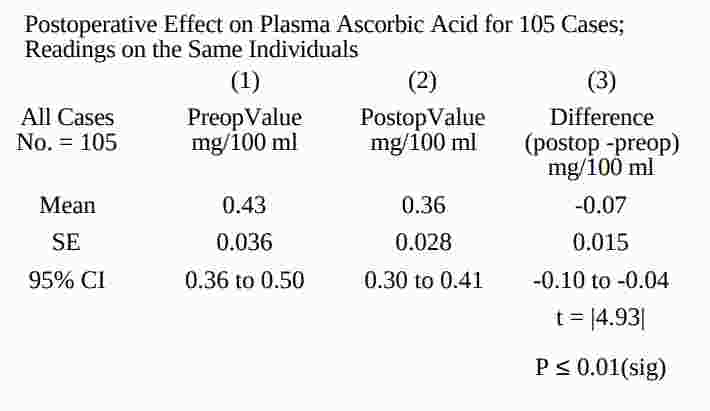
\includegraphics[scale=0.5]{tab3.jpg}
\end{figure}

\begin{enumerate}
\def\labelenumi{\alph{enumi}.}
\tightlist
\item
  \textbf{TRUE (Correct)}
\item
  FALSE
\end{enumerate}

%\showmatmethods


\bibliography{pinp}
\bibliographystyle{jss}



\end{document}

